\documentclass{article}

\usepackage{hyperref}
\hypersetup{
	colorlinks=true,
	linkcolor=blue,
	urlcolor=cyan,}

%%%%%%%%%%%%%%%%%%%%%%%%%%%%%%%%%%%%%%%%%
% Lachaise Assignment
% Structure Specification File
% Version 1.0 (26/6/2018)
%
% This template originates from:
% http://www.LaTeXTemplates.com
%
% Authors:
% Marion Lachaise & François Févotte
% Vel (vel@LaTeXTemplates.com)
%
% License:
% CC BY-NC-SA 3.0 (http://creativecommons.org/licenses/by-nc-sa/3.0/)
% 
%%%%%%%%%%%%%%%%%%%%%%%%%%%%%%%%%%%%%%%%%

%----------------------------------------------------------------------------------------
%	PACKAGES AND OTHER DOCUMENT CONFIGURATIONS
%----------------------------------------------------------------------------------------

\usepackage{amsmath,amsfonts,stmaryrd,amssymb} % Math packages

\usepackage{enumerate} % Custom item numbers for enumerations

\usepackage[ruled]{algorithm2e} % Algorithms

\usepackage[framemethod=tikz]{mdframed} % Allows defining custom boxed/framed environments

\usepackage{listings} % File listings, with syntax highlighting
\lstset{
	basicstyle=\ttfamily, % Typeset listings in monospace font
}

%----------------------------------------------------------------------------------------
%	DOCUMENT MARGINS
%----------------------------------------------------------------------------------------

\usepackage{geometry} % Required for adjusting page dimensions and margins

\geometry{
	paper=a4paper, % Paper size, change to letterpaper for US letter size
	top=2.5cm, % Top margin
	bottom=3cm, % Bottom margin
	left=2.5cm, % Left margin
	right=2.5cm, % Right margin
	headheight=14pt, % Header height
	footskip=1.5cm, % Space from the bottom margin to the baseline of the footer
	headsep=1.2cm, % Space from the top margin to the baseline of the header
	%showframe, % Uncomment to show how the type block is set on the page
}

%----------------------------------------------------------------------------------------
%	FONTS
%----------------------------------------------------------------------------------------

\usepackage[utf8]{inputenc} % Required for inputting international characters
\usepackage[T1]{fontenc} % Output font encoding for international characters

\usepackage{XCharter} % Use the XCharter fonts

%----------------------------------------------------------------------------------------
%	COMMAND LINE ENVIRONMENT
%----------------------------------------------------------------------------------------

% Usage:
% \begin{commandline}
%	\begin{verbatim}
%		$ ls
%		
%		Applications	Desktop	...
%	\end{verbatim}
% \end{commandline}

\mdfdefinestyle{commandline}{
	leftmargin=10pt,
	rightmargin=10pt,
	innerleftmargin=15pt,
	middlelinecolor=black!50!white,
	middlelinewidth=2pt,
	frametitlerule=false,
	backgroundcolor=black!5!white,
	frametitle={Command Line},
	frametitlefont={\normalfont\sffamily\color{white}\hspace{-1em}},
	frametitlebackgroundcolor=black!50!white,
	nobreak,
}

% Define a custom environment for command-line snapshots
\newenvironment{commandline}{
	\medskip
	\begin{mdframed}[style=commandline]
}{
	\end{mdframed}
	\medskip
}

%----------------------------------------------------------------------------------------
%	FILE CONTENTS ENVIRONMENT
%----------------------------------------------------------------------------------------

% Usage:
% \begin{file}[optional filename, defaults to "File"]
%	File contents, for example, with a listings environment
% \end{file}

\mdfdefinestyle{file}{
	innertopmargin=1.6\baselineskip,
	innerbottommargin=0.8\baselineskip,
	topline=false, bottomline=false,
	leftline=false, rightline=false,
	leftmargin=2cm,
	rightmargin=2cm,
	singleextra={%
		\draw[fill=black!10!white](P)++(0,-1.2em)rectangle(P-|O);
		\node[anchor=north west]
		at(P-|O){\ttfamily\mdfilename};
		%
		\def\l{3em}
		\draw(O-|P)++(-\l,0)--++(\l,\l)--(P)--(P-|O)--(O)--cycle;
		\draw(O-|P)++(-\l,0)--++(0,\l)--++(\l,0);
	},
	nobreak,
}

% Define a custom environment for file contents
\newenvironment{file}[1][File]{ % Set the default filename to "File"
	\medskip
	\newcommand{\mdfilename}{#1}
	\begin{mdframed}[style=file]
}{
	\end{mdframed}
	\medskip
}

%----------------------------------------------------------------------------------------
%	NUMBERED QUESTIONS ENVIRONMENT
%----------------------------------------------------------------------------------------

% Usage:
% \begin{question}[optional title]
%	Question contents
% \end{question}

\mdfdefinestyle{question}{
	innertopmargin=1.2\baselineskip,
	innerbottommargin=0.8\baselineskip,
	roundcorner=5pt,
	nobreak,
	singleextra={%
		\draw(P-|O)node[xshift=1em,anchor=west,fill=white,draw,rounded corners=5pt]{%
		Question \theQuestion\questionTitle};
	},
}

\newcounter{Question} % Stores the current question number that gets iterated with each new question

% Define a custom environment for numbered questions
\newenvironment{question}[1][\unskip]{
	\bigskip
	\stepcounter{Question}
	\newcommand{\questionTitle}{~#1}
	\begin{mdframed}[style=question]
}{
	\end{mdframed}
	\medskip
}

%----------------------------------------------------------------------------------------
%	WARNING TEXT ENVIRONMENT
%----------------------------------------------------------------------------------------

% Usage:
% \begin{warn}[optional title, defaults to "Warning:"]
%	Contents
% \end{warn}

\mdfdefinestyle{warning}{
	topline=false, bottomline=false,
	leftline=false, rightline=false,
	nobreak,
	singleextra={%
		\draw(P-|O)++(-0.5em,0)node(tmp1){};
		\draw(P-|O)++(0.5em,0)node(tmp2){};
		\fill[black,rotate around={45:(P-|O)}](tmp1)rectangle(tmp2);
		\node at(P-|O){\color{white}\scriptsize\bf !};
		\draw[very thick](P-|O)++(0,-1em)--(O);%--(O-|P);
	}
}

% Define a custom environment for warning text
\newenvironment{warn}[1][Warning:]{ % Set the default warning to "Warning:"
	\medskip
	\begin{mdframed}[style=warning]
		\noindent{\textbf{#1}}
}{
	\end{mdframed}
}

%----------------------------------------------------------------------------------------
%	INFORMATION ENVIRONMENT
%----------------------------------------------------------------------------------------

% Usage:
% \begin{info}[optional title, defaults to "Info:"]
% 	contents
% 	\end{info}

\mdfdefinestyle{info}{%
	topline=false, bottomline=false,
	leftline=false, rightline=false,
	nobreak,
	singleextra={%
		\fill[black](P-|O)circle[radius=0.4em];
		\node at(P-|O){\color{white}\scriptsize\bf i};
		\draw[very thick](P-|O)++(0,-0.8em)--(O);%--(O-|P);
	}
}

% Define a custom environment for information
\newenvironment{info}[1][Info:]{ % Set the default title to "Info:"
	\medskip
	\begin{mdframed}[style=info]
		\noindent{\textbf{#1}}
}{
	\end{mdframed}
}
 % Include the file specifying the document structure and custom commands

%----------------------------------------------------------------------------------------
%	ASSIGNMENT INFORMATION
%----------------------------------------------------------------------------------------

\title{Project 1: Optical Immunoassay Assignment (OIA)}
\author{BIOE 385 Bioinstrumentation Laboratory} 
\date{}
%----------------------------------------------------------------------------------------

\begin{document}
\large
\maketitle
\section*{Introduction}
You are an engineer working for a Rice University initiated non-profit startup company that is focusing its efforts on developing inexpensive point of care diagnostic systems for use in the developing world. You have been tasked with designing the electronic circuitry for an optical immunoassay system that can test whole blood for many particular analytes without requiring expensive laboratory intensive processing. Fortunately, because Rice University is a haven for nanotechnology research, you can take advantage of nanoshell technology to build such a device. \href{https://github.com/jlongc12/BIOE_385/blob/main/project_1_OIA/immunoassay_article.pdf}{Please see the journal article that explains the technique you will use: \textit{“A Whole Blood Immunoassay Using Gold Nanoshells”}.}\\

If you look carefully at the technique described in the paper, rather than using a spectrophotometer which will test the light transmission through a sample at all wavelengths, your device will simply need to test the light at one wavelength. For a final device, your company may want to run the test at more than one wavelength, but for the purposes of this class, you can prove the concepts with one wavelength. The nanoshells that you will be testing will attenuate light significantly at a wavelength of 850 nm (see \textit{“Spectra of Calibration Samples”} in the course website). The device you make will be housed in a small plastic container with the cuvette held in a film canister and must be portable for physicians or nurses going into the field. A designer has proposed the following for the design:

\begin{figure}[h]
    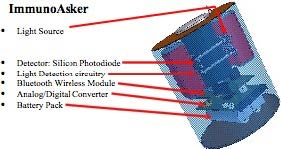
\includegraphics[width=0.8\textwidth]{fig_1.jpg}
    \centering
\caption{Diagram of ImmunoAsker (Courtesy Team Immosaic 2004-2005, Blair Bossart, Ashvin Dewan, Jeffrey
Dietrich, Laura Knezevic, Lisa Justin)}
\label{fig_1}
\end{figure}

\begin{figure}[h]
    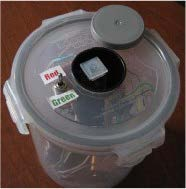
\includegraphics[width=0.6\textwidth]{fig_2.jpg}
    \centering
\caption{Photograph of ImmunoAsker}
\label{fig_2}
\end{figure}

Simply put, you need to build a circuit that contains an LED at the correct wavelength to send a beam of light through your sample in a cuvette and a photodetector to detect your nanoshell aggregation.\\

Since this has not been done previously, you have decided that you need to build and test two possible circuit designs for developing your immunoassay devices. \textbf{After you build detectors from both types of circuit designs}, you will be able to make a recommendation to your boss about how to build the final device.\\

Some things you should consider in making recommendations to your boss: cost, accuracy, difficulty of implementation, and size variation.\\

\section*{Assignment}

\begin{enumerate}
	\item Build a detector using a circuit from the FDS 100 photodetector spec sheet that can be found in the course website.
	\item Build a circuit that will convert current to voltage (see Photodiode signal conditioning circuit example later in this document)
	\item Build a LabView VI to collect data from both circuits so that you can test and troubleshoot them.
	\item Write a good concise report to your boss that contains:
	\begin{enumerate}
		\item Executive summary
		\item Explanation of your goals and methods
		\item Adequate description of your work including:
		\begin{enumerate}
			\item circuit diagrams
			\item theory
			\item component rationale
			\item description and examples of what LabView program can do
		\end{enumerate}
		\item Testing and Results
		\begin{enumerate}
			\item data and plots demonstrating the results obtained
			\item accuracy and precision of each design
		\end{enumerate}
		\item Recommendation for the approach your company should take to develop these devices.
		\begin{enumerate}
			\item limitations of design and possible improvements
		\end{enumerate}
	\end{enumerate}
\end{enumerate}

A Report Grading Rubric for your final report will be available in the course website.\\

This project should be completed before Midterm Recess (see schedule for deadlines). For each week there are a set of guidelines and tasks to complete. However, simply completing the tasks for each week is not enough to be successful in the whole project. Successful completion and true understanding of each task will help you complete the project on time. You are strongly encouraged to look ahead, think about the next steps for the project, and add features you believe would be helpful as you go along. The final week of this section will be a lab test. You can expect to explain and demonstrate your device at your design demonstration.
\end{document}
